
\chapter{Publishing, Interlinking and Querying Geodata}
\label{ch:ch2}

\begin{flushright}
\textit{``If you're a geospatial developer, AJAX is not a domestic cleaning product. \\
If you're a web dev, a polygon is not a dead parrot''}\footnote{\url{http://www.w3.org/2014/03/lgd/report}}.\\
Steve Peters \\
(UK Government's Department \\for Communities and Local Government)

\end{flushright}

\section*{Introduction}
\label{sec:intro-ch2}
So far, the Web of Data has taken advantage of geocoding technologies for publishing large amounts of data. For example, Geonames provides more than 10 millions records (e.g. $5,240,032$ resources of the form \url{http://sws.geonames.org/10000/}) while LinkedGeoData has more than $60,356,364$ triples. All the above mentioned data is diverse in their structure, the access point (SPARQL endpoint, Web service or API), the entities they represent and the vocabularies used for describing them. Table~\ref{tab:srce-data} summarizes for different providers the number of geodata available (resources, triples) and how the data can be accessed.


To publish geospatial data on the Web, some tools are needed for converting native formats into RDF. Those tools are based on OGC libraries for extracting features, and vocabularies provided to build the RDF. Once the dataset obtained, it has to be stored in an efficient way, interconnected to other datasets, and then consumed using SPARQL queries. Moreover, all those steps might be integrated in frameworks that ease the overall process of publishing geodata. In this chapter, we first discuss different representation on the Web of the 7$^{th}$ arrondissement of Paris in DBpedia, Geoname and LinkedGeoData (Section \ref{sec:scenario}). Section \ref{sec:toolgeo} provides an overview of four tools for converting geospatial data into RDF, with a brief discussion on their limitations. Criteria to interlink geodata is then described in Section \ref{sec:interlinking}, followed by a survey on triple stores (Section \ref{sec:surveytps}). We then describe Datalift, a tool for managing the workflow of publishing raw data to RDF (Section \ref{sec:toolLD}), followed by our contributions of publishing French authoritative datasets using Datalift. An evaluation on time execution of built-on geo-functions of three triple stores is presented in Section \ref{sec:geoqueries}, and a brief summary (Section \ref{sec:ch2-summary}) to conclude the chapter.

\section{Current Representation of Geodata on the Web}\label{sec:scenario}
%\section{Scenario: 7$^{th}$ Arrondissement of Paris}                      \label{sec:scenario}
%\todo{Update the scenario with the current version of DBpedia 2014, DBpedia-FR}
In this section, we review the modeling of the 7$^{th}$ arrondissement of Paris, France in different geospatial datasets on the Web. The 7$^{th}$ arrondissement of Paris is one of the 20 arrondissements (administrative districts) of the capital city of France. It includes some of Paris's major tourist attractions such as the Eiffel Tower, some world famous museums (e.g: \textit{mus\'{e}e d'Orsay}) and contains a number of French national institutions, including numerous government ministries\footnote{\url{http://en.wikipedia.org/wiki/7th_arrondissement_of_Paris}}. We use it throughout this paper to highlight the diversity of representations one can use for this geographical entity. We assume that this district should be modeled as a POLYGON composed of a number of POINTs needed to ``interpolate'' its effective boundaries. We assume the use of the WGS84\footnote{\url{http://en.wikipedia.org/wiki/World_Geodetic_System}} geodetic system.

\begin{table}[!htbp]
\centering{
\begin{tabular}{lllc}
 \specialrule{1pt}{1pt}{1pt}
 \textbf{Provider}	 	& {\textbf{\#Geodata}}  & \textbf{Data access}		 \\ \specialrule{1pt}{1pt}{1pt}
DBpedia & 727,232 triples & SPARQL endpoint\\
Geonames & 5,240,032 (feature). &  API \\
LinkedGeoData & 60,356,364 triples & SPARQL endpoint, Snorql\\
Foursquare & N/A & API\\
Freebase & 8,5MB  & RDF Freebase Service\\
Ordnance Survey(Cities) & 6,295 triples  & Talis API \\
GeoLinkedData.es & 101,018 triples  & SPARQL endpoint \\
Google Places & N/A  & Google API \\
GADM   & 682,605 triples & Web Service \\
NUTS  & 316,238 triples & Web Service \\
IGN experimental & 629,716 triples & SPARQL endpoint \\
LOD Greek & 634 KTriples & SPARQL endpoint \\
 \specialrule{1pt}{1pt}{1pt}
\end{tabular}
\caption{Geodata by provider and their different access type, either API, Web service or SPARQL endpoint.}
\label{tab:srce-data}
}
\end{table}

\subsection{DBpedia Modeling}
We provide below an excerpt of the DBpedia 3.8 description for the same resource:
{\small
\begin{verbatim}
  dbpedia:7th_arrondissement_of_Paris a gml:_Feature ;
    a <http://dbpedia.org/class/yago/1900SummerOlympicVenuEs>
    rdfs:label "7. arrondissementti (Pariisi)"@fi; (14 different languages)
    dbpprop:commune "Paris" ;
    dbpprop:departement  dbpedia:Paris ;
    dbpprop:region dbpedia:Ile-de-France_(region) ;
    grs:point "48.85916666666667 2.312777777777778" ;
    geo:geometry "POINT(2.31278 48.8592)" ;
    geo:lat "48.859165"^^xsd:float;
    geo:long "2.312778"^^xsd:float.
\end{verbatim}
}
First, we observe that the type \texttt{gml:\_Feature} and the property \texttt{grs:point} are not resolvable since there are no OWL ontologies that provide a description of them. Second, the property \texttt{geo:geometry} used by DBpedia is not defined in the WGS84 vocabulary. For the geometry, the 7th arrondissement is a simple POINT defined by a latitude and a longitude.

\subsection{Geonames Modeling}
In Geonames, the 7$^{th}$ arrondissement is considered as a 3$^{rd}$ order administrative division, represented by a POINT for the geometry model. The RDF description of this resource gives other information such as the alternate name in French, the country code and the number of inhabitants.
{\small
\begin{verbatim}
  gnr:6618613 a gn:Feature ;
    gn:name "Paris 07";
    gn:alternateName "7ème arrondissement";
    gn:featureClass gn:A [
      a skos:ConceptScheme ;
      rdfs:comment "country, state, region ..."@en .
    ] ;
    gn:featureCode gn:A.ADM4 [
      a skos:Concept ;
      rdfs:comment "a subdivision of a 3rd order admin division"@en .
    ];
    gn:countryCode "FR";
    gn:population "57410";
    geo:lat "48.8565";
    geo:long "2.321".
\end{verbatim}
}

\subsection{LinkedGeoData Modeling}
In LinkedGeoData dataset, the district is a \texttt{lgdo:Suburb} which is  subClass of \texttt{ldgo:Place}. Its geometry is still modeled as a POINT and not as a complex geometry of type POLYGON as we could have expected for this type of spatial object.
{\small
\begin{verbatim}
  lgd:node248177663 a lgdo:Suburb ;
    rdfs:label "7th Arrondissement"@en , "7e Arrondissement" ;
    lgdo:contributor lgd:user13442 ;
    lgdo:ref%3AINSEE 75107 ;
    lgdp:alt_name "VIIe Arrondissement" ;
    georss:point "48.8570281 2.3201953" ;
    geo:lat 48.8570281 ;
    geo:long 2.3201953 .
\end{verbatim}
}

\subsection{Discussion}
These samples from DBpedia, Geonames and LinkedGeoData give an overview of the different views of the same reality, in this case the district of the 7$^{th}$ Arrondissement in Paris. Regarding the ``symbolic representation'', two datasets opted for ``Feature'' (DBpedia and Geonames) while LGD classifies it as a ``Suburb'' or ``Place''. They all represent the shape of the district as a POINT which is not very efficient if we consider a query such as \emph{show all monuments located within the 7th arrondissement of international importance}. To address this type of query and more complicated ones, there is a need for more advanced modeling as we describe in the next section.

\section{Existing Tools for Converting Geospatial Data}
\label{sec:toolgeo}
To address the need for converting geodata into a graph model such as RDF, there are some tools that have been proposed to generate RDF data from legacy geospatial datasets. The differences among the tools are based on four main criteria :
\begin{itemize}
\item \textbf{Input format:} The different types of formats accepted as input of the tool;
\item \textbf{Vocabulary:} The vocabulary used to handle the geometry aspect of the spatial data during the RDF conversion step;
\item \textbf{CRS converter:} The presence or not of a CRS converter between different CRSs in the final output of the tool ;
\item \textbf{Output:} The type of serialization in RDF, and more importantly the choice between structured geometry, OGC compliant (WKT, GML literals) or both for the geometry part of the features.
\end{itemize}

Almost all the tools use the OGC libraries for parsing and extracting features from shape formats, such as GDAL (Geospatial Data Abstraction Library) and GeoTools.

\subsection{Geometry2RDF} \label{sec:geo2rdf}
Geometry2RDF \cite{deLeon2010} is a java based tool\footnote{\url{https://github.com/boricles/geometry2rdf}} that generates RDF triples from geometrical information, which can be available in GML or WKT. The tool takes as input any ESRI shapefiles, spatial DBMS (Oracle,  PostgreSQL, MySQL, etc), transforms into GML (using GeoTools\footnote{\url{http://www.geotools.org}}) and then generates RDF (using Jena\footnote{\url{https://jena.apache.org/}}) consistent with the NeoGeo vocabulary. The default CRS used for the geometry is WGS84. The architecture is flexible to run as a standalone platform or as a library.

\subsection{TripleGeo}
TripleGeo \cite{triplegeo2014} is an ETL (Extract- Transform-Load) tool derived from Geometry2RDF (Cf. Section \ref{sec:geo2rdf}) to transform a variety of geospatial databases and shapefiles (including KML and INSPIRE compliant files) into RDF triples. Triples can be exported according to the GeoSPAQL standard, the WGS84 vocabulary and the Virtuoso RDF vocabulary\footnote{\url{http://docs.openlinksw.com/virtuoso/rdfsparqlgeospat.html}}. In addition TripleGeo allows on-the-fly reprojection between CRSs, e.g., transform geometries from GreekGrid87 (a local CRS) into WGS84 (used for GPS locations). The code is available at \url{https://github.com/GeoKnow/TripleGeo}.

\subsection{shp2GeoSPARQL}
shp2GeoSPARQL \cite{saavedra14} is also an extension of Geometry2DF which transforms Shapefiles into RDF in the cadastral domain using ISO 19152 \cite{iso2012} (Land Administration Domain Model) and GeoSPARQL. The geometries obtained by shp2GeoSPARQL are consistent with the GeoSPARQL geometry vocabulary.


\subsection{GeomRDF: Datalift tool for Converting Geodata}
\label{sec:geomRDF}
GeomRDF \cite{hamdi14} is a tool developed within the Datalift platform that transforms geospatial dataset from traditional GIS formats into RDF, and overcome the limitations of the existing tools mentioned in Section \ref{sec:limitations}. GeoRDF is based on a vocabulary that reuses and extends GeoSPARQL and NeoGeo so that geometries can be defined in any CRS, and represented both as structured geometries and GeoSPARQL standard compliant. \geom is composed of three components:

\begin{itemize}
\item \textbf{input parsers:} This component extracts from the different input format all the features and their descriptions.
\item \textbf{feature parsers:} This component extracts for all the features their properties depending on their type, either thematic (attributes and properties of a geographic entity) or geometric (the geometry associated to the entity). For example, in the case of a Multipolygon, the parser stores first all the Polygons composing the original Multipolygon. Then, it stores the exterior and the eventual LinearRings for each Polygon, as well as the points included in the LinearRings. Finally the coordinates of each point are also stored. At this stage, GeoRDF provides a \textit{``CRS reprojection''} functionality, which consists of transforming on-the-fly between different CRSs, before the storage of the geometries.

\item  \textbf{RDF Builder:} This module is in charge of generating RDF triples according to the \texttt{geom} vocabulary for geometry, \textbf{geofla} and \textbf{topo} for different topographic entities.


\end{itemize}

GeomRDF is implemented as a module of the RDF publication platform Datalift. Moreover, it has been validated against the French Administrative Units dataset. GeomRDF can also can also bee used as a stand-alone library and can be accessed at \url{https://github.com/fhamdi/GeomRDF}. Listing \ref{lst:nicegeomrdf} presents a snippet in TURTLE of GeomRDF for geometry of the city of Nice (France). It also contains the structured modeling of a MultiPolygon as a set of Polygon, containing Points in an LinearRing.



 \begin{lstlisting}[label=lst:nicegeomrdf, float=tp, numbers=left, numberstyle=\tiny, caption = Sample of structured geometry of the city of Nice]
@prefix geom:<http://data.ign.fr/def/geometrie#> .
@prefix rgeofla:<http://data.ign.fr/id/geofla/commune/> .
@orefix gsp: <http://www.opengis.net/ont/geosparql#> .

rgeofla:Multipolygon_11130 a geom:MultiPolygon ;
geom:crs <http://data.ign.fr/id/ignf/crs/WGS84GDD> ;
geom:polygonMember _:polygon_11130_1 ;
geom:polygonMember _:polygon_11130_2 .

_:polygon_11130_1 a geom:Polygon ;
geom:crs <http://data.ign.fr/id/ignf/crs/WGS84GDD> ;
geom:exterior  _:linearRing_11130_1 .

_:polygon_11130_2 a geom:Polygon ;
geom:crs <http://data.ign.fr/id/ignf/crs/WGS84GDD> ;
geom:exterior  _:linearRing_11130_2 .


_:linearRing_11130_1 a geom:LinearRing ;
geom:crs <http://data.ign.fr/id/ignf/crs/WGS84GDD> ;
geom:points  _:points_11130_1 ;
geom:firstAndLast _:point_11130_10 .


_:linearRing_11130_2 a geom:LinearRing ;
geom:crs <http://data.ign.fr/id/ignf/crs/WGS84GDD> ;
geom:points  _:points_11130_2 ;
geom:firstAndLast _:point_11130_2 .


_:points_11130_1 a geom:PointsList; geom:firstAndLast _:point_11130_10 ;
rdf:rest _:point_11130_11 .
_:point_11130_11  a geom:PointsList; rdf:first _:point_11130_12 ;
rdf:rest _:point_11130_13 .
.....
_:point_11130_129  a geom:PointsList; rdf:first _:point_11130_130 ;
rdf:rest _:point_11130_1 .


_:point_11130_10 a geom:Point ;
geom:crs <http://data.ign.fr/id/ignf/crs/WGS84GDD> ;
geom:coordX "7.308745254207776"^^xsd:double ;
geom:coordY "43.69237084089203"^^xsd:double .

rgeofla:06088  a geofla:Commune ;
rdfs:label "NICE"@fr ;
geom:geometry rgeofla:Multipolygon_11130 ;
gsp:asWKT "<http://data.ign.fr/id/ignf/crs/WGS84GDD> MULTIPOLYGON (((7.308745254207776 43.69237084089203, 7.306051040744396 43.68445728916297, ....., 7.308745254207776 43.69237084089203)))"^^gsp:wktLiteral .

\end{lstlisting}


\subsection{Limitations of existing tools}
\label{sec:limitations}

Currently, the tools achieving the transformations of geospatial data into RDF still suffer from some limitations. On one hand, they are all compatible with GeoSPARQL standard, which in turns has a handful endpoints that implements all the requirements. Moreover, geometries are literals (e.g., wktLiteral, gmlLiteral) with embedded CRS. On the other hand, tools based on NeoGeo vocabulary outputs structured geometries that can be easily handled by existing Triple Stores and SPARQL queries. However, NeoGeo only allows geometry in WGS84 CRS. The ideal scenario could be a tool that provides output consistent with both GeoSPARQL and structured geometries handling multiple CRSs.
Figure \ref{fig:shape2rdf-generic} shows a generic architecture for tools to convert ESRI ShapeFiles into different flavor of RDF. Tools differ mainly in the presence or not of the CRS reprojection, the vocabularies used for the RDF output, and the compatibility with GML and WKT representations.

\begin{figure}[ht!b]
\centering{
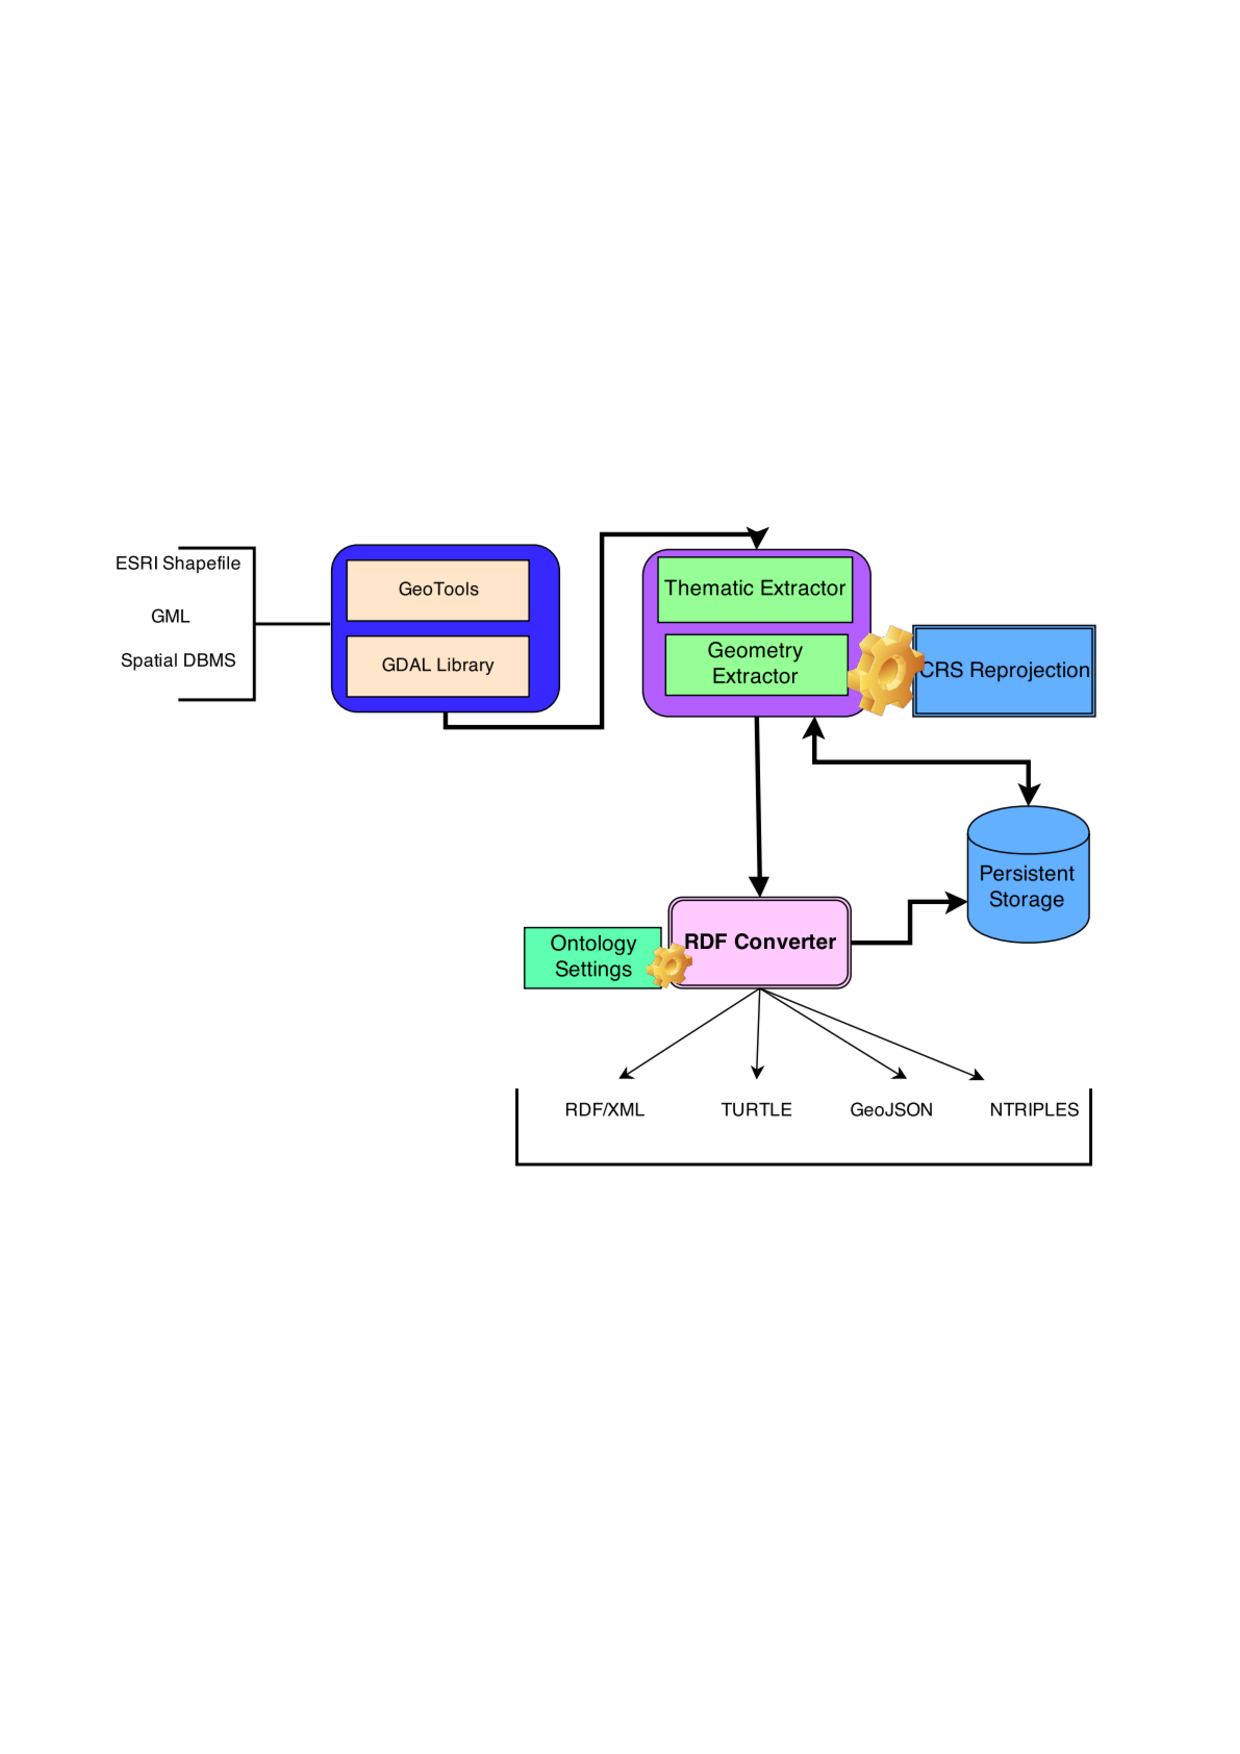
\includegraphics[scale=0.7]{img/shape2rdf-generic.pdf}
\label{fig:shape2rdf-generic}
\caption{Generic architecture of tools for converting raw geospatial data into RDF.}
}
\end{figure}


\section{Interlinking Geospatial Vocabulary and Data}
\label{sec:interlinking}

We present in this section different criteria that can be used to interlink geospatial datasets in the context of Web of Data, as well as some distance measures adapted for combining two geospatial datasets. We first provide results of aligning two existing ontologies of previous project GeOnto with five ontologies and two flat taxonomies containing geospatial. For more details on mapping techniques, the readers can refer to \cite{euzenat2007}, and functions implemented in SILK \cite{jentzsch2010silk,isele2011} and LIMES \cite{ngau11} interlinking tools. Among the set of properties usually used as data linking criteria, geolocation (addresses, postal code, latitude/longitude, etc) remains one of the most commonly used.

In this thesis, our linking approach is mainly based on geolocation properties comparison, although is by either combining well-known functions implemented in SILK and LIMES. The result of this interlinking process is a list of \textit{``owl:sameAs''} links between entities of each datasets, with a certain score.

\subsection{Schema Alignment of Existing Vocabularies}                                         \label{sec:vocabalignment}
%IGN is a public service in France in charge of describing, from the physical and geometry point of view, the surface of the French territory and the occupation of the land, and to elaborate and update continuously the forestal resources. They are also experimenting in exposing some of their data as Linked Data and act as an important provider in the \url{http://data.gouv.fr} portal.
IGN-France has previously developed two complementary vocabularies (GeOnto and bdtopo) which differ in their provenance but have the same scope, for describing geographic entities in the French territory. GeOnto is the product of a French research project\footnote{\url{http://geonto.lri.fr/Livrables.html}} aiming at building and aligning heterogeneous ontologies in the geographic domain. A ``light'' version of the final ontology at \url{http://semantics.eurecom.fr/datalift/tc2012/vocabs/GeoOnto/} defines two high level classes in a total of $783$ classes and $17$ properties ($12$ Data Properties and $5$ Object Properties). GeOnto contains labels in both French and English, without comments specified for the terms. The bdtopo ontology is derived from a geospatial database with the same name. It contains $237$ classes and $51$ properties ($47$ DP / $4$ OP). All the labels and comments are in French.

\subsubsection{GeOnto Alignment Process: First results}
The first step towards interoperability of French geographic features and the existing vocabularies is to align GeOnto to other vocabularies. We choose GeOnto because it covers a large number of categories and also has labels in English. We have performed the alignment with five OWL vocabularies (bdtopo, LGD, DBpedia, Schema.org and Geonames) and two flat taxonomies (Foursquare, Google Place). For the latter, we have transformed the flat list of types and categories into an OWL ontology. For each alignment performed, we only consider \texttt{owl:equivalentClass} axioms. We use the Silk tool \cite{Julius09} to compute the alignment using two metrics for string comparison: the \textit{levenshteinDistance} and \textit{jaro} distances. They work on the English labels except for the alignment with bdtopo where we use the French labels. We apply the average aggregation function on these metrics with an empirically derived threshold. However, for generating the final mapping file for vocabularies of small size, we manually validate and insert relations of type \texttt{rdfs:subClassOf}. The threshold to validate the results is set to $100$\% for links considered to be correct and greater than $40$\% for links to be verified. The alignment with Geonames is special, considering the property restriction used in the ontology for codes.

Table~\ref{tab:mappings} summarizes the result of the alignment process between GeOnto and the existing vocabularies and taxonomies. All the resources of this work are available at \url{http://semantics.eurecom.fr/datalift/tc2012/}.
\begin{table}
\centering{
\begin{tabularx}{\textwidth}{|X|X|r|}%{|l|l|c|}
\hline
\textbf{Vocabulary}    	& \textbf{\#Classes} 	& \textbf{\#Aligned Classes}    \\ \hline
LGD 			& \texttt{owl:Class}:$1294$     &  $178$			            \\  \hline

DBpedia     	& \texttt{owl:Class}:$366$ 	    & $42$			   				 \\ \hline
				
Schema.org 		& \texttt{owl:Class}:$296$ 	    &  $52$			     			 \\ \hline
				
Geonames		& \texttt{skos:ConceptScheme}:$12$  &  --			    	 	  \\
               	& \texttt{skos:Concept}:$699$       &  $287$               			\\ \hline
Foursquare 		& $359$ 	    			        & $46$ 			 			   \\ \hline
Google Place 	& $126$ 	  			            & $41$ 			 	 			\\ \hline
bdtopo 			& \texttt{owl:Class}:$237$ 	  	    & $153$ 			 	 		\\ \hline
\end{tabularx}
\caption{Results of the alignment process between GeOnto and existing vocabularies/taxonomies.}
\label{tab:mappings}
}
\end{table}

In general, we obtain good results with Silk, with precision beyond $80$\%: Google Place: $94$\%, LGD: $98$\%, DBpedia: $89$\%, Foursquare: $92$\% , Geonames: $87$\% and bdtopo: $92$\%. We obtained a precision of only $50$\% with schema.org due to numerous fine-grained categories that are badly aligned (e.g. \texttt{ign:Berge owl:equivalentClass schema:Park}).


\subsection{Criteria for interlinking geospatial Data}
Data interlinking task is generally performed by comparing properties values of each resource of a source dataset with corresponding properties of the resources described in the target datasets \cite{scharffe2010}. In the field of geographic databases, data matching is also performed by comparing properties, and especially geometries (points, lines, polygons, etc.) that are used to represent the shape and the location of geographic features. This task is usually based on distance measures chosen according to the type of the geometric primitives that must be compared \cite{mustiere2008,anamaria08,Julius09,walter1999}.


In \cite{anamaria08}, the author mentions many different forms of interlinking geospatial datasets. We highlight below some of the most important criteria to be taken into account in the process of interlinking two geospatial datasets:
\begin{itemize}
\item \textbf{Geometrical criteria:} This criteria is based on the geometry of the objects, which is very specific to geographic data. In general, geometry refers to the location and the implicit information regarding the shape(length, orientation, etc.).
\item \textbf{Topological criteria:}
Topology describes the relations of inclusion between objects and use the notion of neighborhood. Topological relationships are used for relations such as: the forest borders the road, two roads are connected, etc. Topological relationships are created from the geometry of the initial geographical objects.
\item \textbf{Attributes criteria:} This criteria uses different attributes belonging to the geographical object, such as name, nature or number of ways. As illustrated in Figure \ref{fig:geomObject}, the attributes of a geographic object can be quantitative or qualitative. The nature of the geographical object is the most important attribute to use in the process of interlinking geospatial data \cite{anamaria08}. This motivates the creation of domain ontologies to provide context in the process of interlinking, where domain-specific ontology alignment frameworks such as TaxoMap \cite{reynaud2007,hamdi2010} gives good precision for a large topographic ontology.

\end{itemize}

\begin{figure}[ht!b]
\centering{
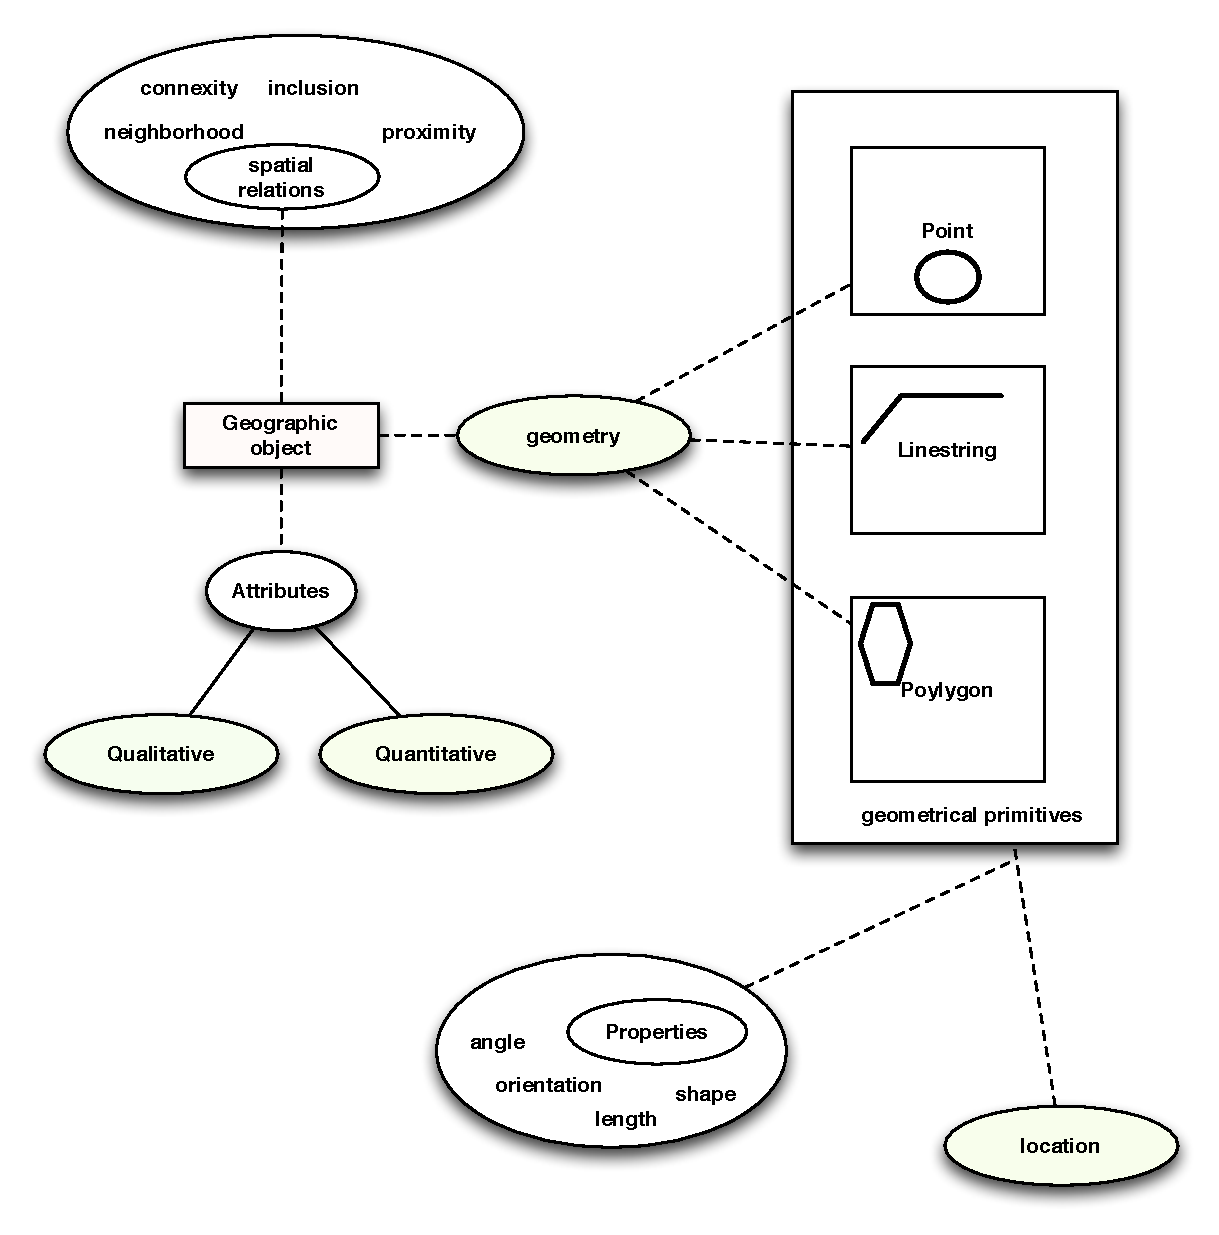
\includegraphics[scale=0.65]{img/geometric-object.pdf}
\label{fig:geomObject}
\caption{Features of a geographic object adapted from \cite{anamaria08}.}
}
\end{figure}

\subsection{Functions for Comparing Geometries}
%\todo{only describe distance and hausdorff -see these anamaria08}
%\todo{add table for distance functions implemented in SILK and LIMES, and compare them?} \\
\paragraph{Euclidean Distance:}
For two objects represented with points, the principal distance used  for measuring their position is the euclidean distance (see Figure \ref{fig:geodistances}). Considering two objects $O_{1} = (x_{1}, y_{1})$ and $O_{2} = (x_{2}, y_{2})$, the euclidean distance $dy_{E}$ between the two objects is defined as follows:
\begin{equation}
d_{E} = \sqrt{((x_{1} - x_{2})^2 + ((y_{1} - y_{2})^2}
\end{equation}


\begin{figure}[ht!b]
\centering{
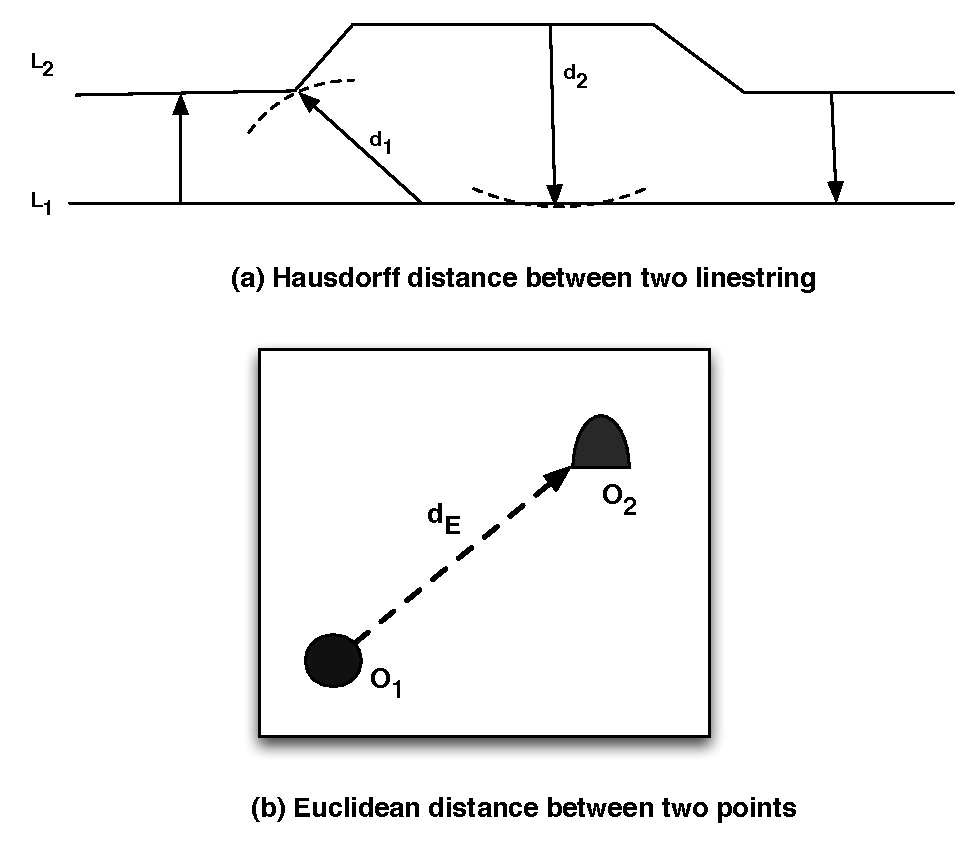
\includegraphics[scale=0.65]{img/geodistances.pdf}
\label{fig:geodistances}
\caption{The most used distances on geometries: (a) the euclidean distance and (b) the Hausdorff distance.}
}
\end{figure}


\paragraph{Hausdorff distance:}
For complex geometries (polylines, linestring, polygones, etc.) there are different measures in the literature, such as mean distance, Fr\'echet distance and Hausdorff distance \cite{anamaria08}. However, at the time of writing this thesis, a Hausdorff distance measure is mostly used in LIMES framework for complex geometries. Considering two linestrings $L_{1}$ and $L_{2}$, the Hausdorff distance represents the maximal distance between the two lines according to the following equation:
\begin{equation}
d_{H} = max(d_{1}, d_{2} )
\end{equation}
where $d_{1}$ and $d_{2}$ are defined as follows:


\begin{align}
d_{1} = max_{p_{1} \in L_{1}}[min_{p_{2} \in L_{2}}[d_{E}(p_{1}, p_{2})]] \\
d_{2} = max_{p_{2} \in L_{2}}{p_{2}}[min_{p_{1} \in L_{1}}[d_{E}(p_{2}, p_{1})]]
\end{align}



Currently on the Web of Data, resources that actually refer to complex topographic features are generally described by very simple geolocation properties, such as a position defined by coordinates (longitude, latitude). On the other hand, geographic reference datasets provide more precise geometric information about geographic features. Interlinking thematic Linked Open Datasets with geographic reference datasets enable to take advantage of both information sources to link independent thematic datasets and create rich cartographic applications for data visualization \cite{feliachi2013}.


\section{Survey on Triple Stores}
\label{sec:surveytps}

A triple store is a back-end that has some form of persistent storage of RDF data and provides mechanisms to run SPARQL \cite{sparql11} queries against that data. The SPARQL support can either be built-in as part of the main tool, or an add-on installed separately. In this section, we discuss the most used triple stores based on the list maintained by sparqles \cite{sparqles13} and we classify them in two group: (i) ``generic triple stores'' that handle any RDF triples and (ii) ``geospatial triple stores'', the ones designed to handle geographic data and implement topological functions.


\subsection{Generic Triple Stores}
\label{sec:genrictps}

We briefly describes some well-known triple stores that has proven to have passed the ``10 Billion Statements'', that is they are able to load and handle more than 10 billion of triples.
\subsubsection{Virtuoso}
Virtuoso is a triple store developed by OpenLink\footnote{\url{http://virtuoso.openlinksw.com/}} and releases both in Open source and commercial versions. It implements part of SPARQL1.1 and store billion of triples. The geospatial extension implements subset of SQL MM functions. A geometry stores in Virtuoso uses a special RDF typed literal \texttt{virtrdf:Geometry}\footnote{\url{http://www.openlinksw.com/schemas/virtrdf\#}}. Such a literal is automatically indexed in an R tree index. Only geometry in WGS84 can be manipulated. Virtuoso is used as back-end for one of the most used dataset in the LOD cloud, \textsc{DBPEDIA}\footnote{http://dbpedia.org/sparql}


\subsubsection{OWLIM}
OWLIM is a semantic repository developed by Ontotext\footnote{\url{http://www.ontotext.com/owlim}}, which provides support and querying of
two-dimensional point geometries modeled with the W3C Geo vocabulary. It implements spatial predicates represented as property funcions. The available four operations are: Buffer, Distance, Nearby and Point-in-polygon. OWLIM is implemented as a storage and inference layer for Sesame, with custom spatial index.

\subsubsection{AllegroGraph}
AllegroGraph\footnote{\url{http://franz.com/agraph/allegrograph/}} is another RDF store developed and maintained by Franz Inc. which stores geospatial data types as native data structures. Support is provided both for Cartesian coordinate systems and for spherical coordinate systems. Every datum in an AllegroGraph store is a UPI, and for geospatial data, the added UPI type is \texttt{:geospatial} with type code \texttt{+geospatial+}. Geometries are assigned to geometric objects through the use of property \url{<http://franz.com/ns/allegrograph/3.0/geospatial/pos>}, and for querying a GEO operator is introduced to express geospatial query patterns in SPARQL. AllegroGraph provides some operations on geodata, such as Bounding Box, Distance and Buffer.




\subsection{Geospatial Triple Stores}
\label{sec:geotps}
We discuss in this section two triple stores built for indexing and querying geospatial data, Parliament and Strabon. We acknowledge that there might be some other solutions (e.g., Oracle DBMS version 111g, release 2). More details can be found in \cite{koubarakis12, battle12, garbis13}. In \cite{garbis13}, the authors present a benchmark of Geospatial RDF stores in the context of the TELIOS project\footnote{http://geographica.di.uoa.gr}, which uses real-world and synthetic data to test the offered functionality and the performance of some prominent geospatial RDF stores.

\subsubsection{Parliament}
\
The RDF store Parliament\footnote{\url{http://parliament.semwebcentral.org}} developed by BBN Technologies fully implements most of the functionality of GeoSPARQL \cite{battle12}.
Parliament has been extended to provide the first implementation of GeoSPARQL, therefore geometries are represented using the WKT and GML serializations.
Therefore, topological functions belonging in the OGC Simple Feature Access, Egenhofer and RCC8 families are exposed by Parliament.
Topological properties and non-topological functions are also available.In addition, multiple coordinate reference systems may be used. Parliament is implemented in C++, and Java Native Interface is used to couple with Jena, and includes a rule engine, serving as a means of inference. It registers the presence of a spatial object in an R-Tree.

\subsubsection{Strabon}
%\todo{read again the paper}
Strabon\footnote{\url{http://www.strabon.di.uoa.gr}} is a semantic spatio-temporal RDF store for \texttt{stRDF}\footnote{\url{http://strdf.di.uoa.gr/ontology}} and \texttt{stSPARQL} \cite{strabon12}. Strabon extends the well-known RDF store Sesame\footnote{\url{http://rdf4j.org/}}, allowing it to manage both thematic and spatial data expressed in \texttt{stRDF}. PostGIS is used as the relational backend of Strabon.
stRDF uses OGC standards (the OGC SFA specification in particular) for the representation of geospatial data.
The datatypes strdf:WKT and strdf:GML are introduced to represent geometries serialized using the OGC standards WKT and GML. Strabon allows geometries to be expressed in any coordinate reference system defined by the EPSG (European Petroleum Survey Group) or OGC. In addition, the latest version of Strabon implements the GeoSPARQL Core, Geometry extension and Geometry topology extension components.


%\begin{table}[!htbp]
 %\begin{tabularx}{\textwidth}{|X|X|X|X|X|l|}
 %\hline
 %\textbf{Triple store} & WKT-compliance & GML-compliance & Geometry supported  & Geospatial Functions & GeoVocab \\ \hline
% Virtuoso & Yes & Yes & Point & 13 functions & W3C Geo + Typed Literal  %\\ \hline
% Allegro-Graph & \-- & -- & Point & 3 functions & ``strip'' mapping data \\ \hline
% OWLIM-SE & -- & -- & Point & 4 functions & W3C Geo\\ \hline
%Open Sahara & \ Yes & Yes & Point, Line, Polygons & 23 functions  & Typed Literal \\ \hline
% Parliament & \ Yes & Yes & Point, Line, Polygons & 23 functions  &  GeoSPARQL vocabulary\\ \hline
% \end{tabularx}
%\caption{Triple stores survey with respect to geometry types supported and geospatial functions implemented.}
%\label{tab:triplestore}
%\end{table}

\subsection{Assessing Triple Stores }
%\todo{update the table with strabon and changes in virtuoso 7.} \\
There are many criteria that can be used to assess triple stores based on the requirements dataset publishers. Most importantly are the compatibility with the set of standards for RDF and SPARQL (e.g., SPARQL1.0, SPARQL1.1). Table \ref{tab:generictriples} provides an overview comparing ``generic'' triple stores. Currently, none of the triple stores listed supports security mechanisms built natively. Regarding specific geospatial triple stores (or extensions of geospatial in RDF stores), more specific requirements are needed to index and provide native functions/operations over geometries. In Table \ref{tab:generictriples}, triple stores are compared based on the following features:

\begin{itemize}
\item the types of geometries supported,
\item the coverage of spatial functions,
\item the compliance with GeoSPARQL standard,
\item the extensions to existing vocabularies and SPARQL to manage geodata.
\end{itemize}

\begin{table}[htb!]
    \caption{Survey of some generic popular triple stores.}
    \label{tab:generictriples}
    \centering
    \begin{tabular}{lllllll}
    \toprule
    \textbf{Feature} & \textbf{Virtuoso} & \textbf{OWLIM} & \textbf{AllegroGraph} & \textbf{4Store} &  \textbf{Sesame} & \textbf{Fuseki} \\
    \toprule
    \texttt{SPARQL1.0} & Yes & Yes & Yes & Yes & Yes & Yes \\
    \midrule
    \texttt{SPARQL1.1} & Partial & Yes & Partial & Partial & Partial & Yes \\
    \midrule
    \texttt{SPARQL Update} & Non-std & Yes & Yes & Yes & Yes & Yes \\
    \midrule
    \texttt{Reasoning} & Rules & Rules & Rules & Add-on & Little & Rules \\
    \midrule
    \texttt{10 billion statements} & Yes & Yes & Yes & No & No & No \\
    \midrule
    \texttt{Clustering} & Yes & Yes & Yes & Yes & No & No \\
    \midrule
    \texttt{Open source} & Yes & No & No & Yes & Yes & Yes \\
    \bottomrule
    \end{tabular}
\end{table}

\paragraph{Serialization and Triple stores:} We also advocate the use of properties that can provide compatibility with other formats (GML, KML, etc.). This choice can be triple store independent, as there could be ways to use content-negotiation to reach the same result. In Table \ref{tab:triplestore}, \texttt{Open Sahara}, \texttt{Parliament } and  \texttt{Virtuoso} are WKT/GML-compliant with respectively $23$ and $13$ functions dealing with geodata. Moreover, the choice of the triple store (e.g.,Virtuoso\footnote{Here we used Virtuoso Open Edition, V6.xx} vs Open Sahara) is not really an issue, as the IndexingSail\footnote{\url{https://dev.opensahara.com/projects/useekm/wiki/IndexingSail}} service could also be wrapped on-top of Virtuoso to support full OpenGIS Simple Features functions\footnote{\url{http://www.opengeospatial.org/standards/sfs}}.

\begin{table}[ht!bp]
  \caption{Triple stores survey with respect to geometry types supported and geospatial functions implemented.}
  \label{tab:triplestore}
  \centering
  \begin{tabular}{lll}
    \toprule
    \textbf{Triplestore} & \textbf{WKT-Compliance } &  \textbf{GML-Compliance } \\
    \textbf{Geometry supported} & \textbf{Geospatial Functions} &  \textbf{Geo-vocabulary} \\
    \toprule
    \texttt{Virtuoso} & Yes & Yes \\
    Point & SQL/MM (subset) & W3C Geo + Typed Literal \\
    \midrule
    \texttt{AllegroGraph} & \-- & \-- \\
    Point & Buffer, Bounding Box, Distance & ``strip'' mapping data \\
    \midrule
    \texttt{OWLIM-SE} & N/A & N/A \\
    Point & Distance, Buffer, Nearby, Within & W3C Geo \\
    \midrule
    \texttt{Open Sahara} & \ Yes & Yes \\
    Point, Line, Polygons & OGC-SFA, Egenhofer, RCC-8 & Typed Literal \\
    \midrule
    \texttt{Parliament} & \ Yes & Yes \\
    Point, Line, Polygons & OGC-SFA, Egenhofer, RCC-8 &  GeoSPARQL vocabulary\\
    \midrule
    \texttt{Strabon} & \ Yes & Yes \\
    Point, Line, Polygons & OGC-SFA, Egenhofer, RCC-8 &  stRDF\\
    \bottomrule
  \end{tabular}
\end{table}

%\subsection{Benchmarks for Geospatial RDF Stores}



\section{Datalift: A tool for Managing Linked (Geo)Data Publishing Workflow}
\label{sec:toolLD}
In this section, we present the Datalift platform, as a tool to help for lifting raw data to RDF. existing tools that manage the workflow of publishing geodata on the Web. To the best of our knowledge, a related framework providing similar functionalities is the \textsc{Geoknow Stack} that we discuss in section \ref{sec:geoknow}.

\subsection{Datalift Platform}
\label{sec:datalift}
Datalift is an open source platform \cite{scharffe_2012} helping to lift raw data sources or legacy data to semantic interlinked data sources.
The ambition of DataLift is to act as a catalyst for the emergence of the Web of Data by providing a complete path from raw data to fully interlinked, identified, and qualified linked datasets. The Datalift platform supports the following stages in lifting the data:
\begin{enumerate}
\item Selection of ontologies for publishing data;
\item Conversion of data to the appropriate format (e.g., from CSV to RDF);
\item Interlinking of data with other data sources;
\item Publication of linked data ;
\item Access control and license management.
\end{enumerate}

Figure \ref{fig:liftprocess} gives an overview of the different steps in lifting raw source data into RDF using different modules of Datalift.

\begin{figure}[!htp]
\centering{
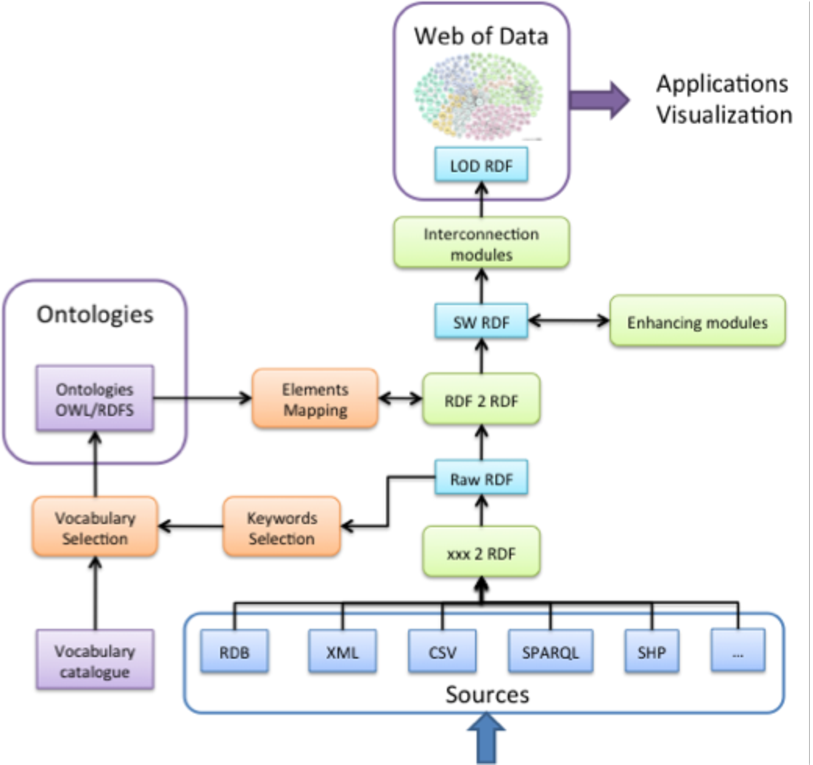
\includegraphics[scale=0.7]{img/liftProcessDatalift.pdf}
\caption{Lifting process of raw data source into RDF using Datalift Platform}
\label{fig:liftprocess}
}
\end{figure}


\subsubsection{Functionalities of the Datalift platform}

The architecture of Datalift is modular. Several levels of abstraction allow decoupling between the different stages from raw data to semantic data. The dataset selection allows us to identify the data to be published and migrate them to a first RDF version. The ontologies selection step asks the user to input a set of vocabularies', terms that will be used to describe the lifted data. Once the terms are selected, they can be mapped to the raw RDF and then converted to properly formatted RDF. The data is then published on the DataLift SPARQL endpoint. Finally, the process aims at providing links from the newly published data to other datasets already published as Linked Data on the Web. Figure \ref{fig:liftprocess} corresponds to a visual depiction of the workflow to convert raw data into \textit{``structured''} RDF data. Figure \ref{fig:dataliftarch} depicts the architecture of Datalift, consisting of different modules for:

\begin{figure}[ht!b]
\centering{
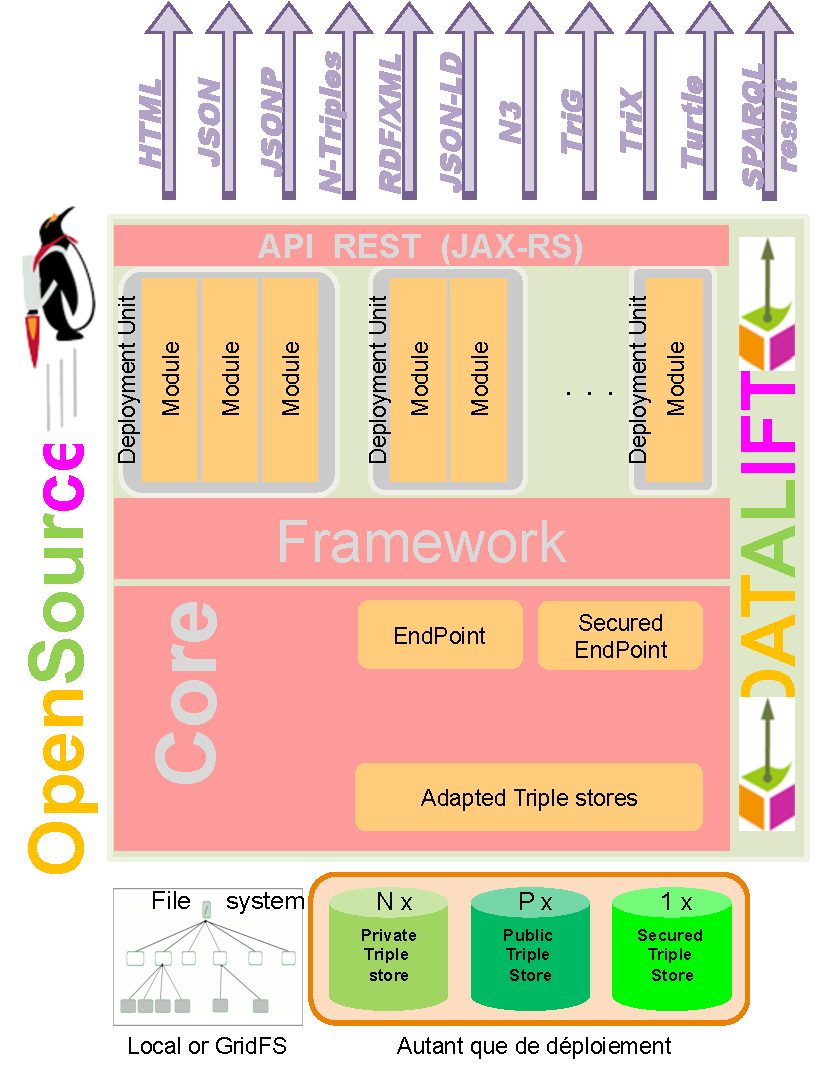
\includegraphics[scale=0.6]{img/datalift-architecture.pdf}
\label{fig:dataliftarch}
\caption{Architecture of Datalift platform.}
}
\end{figure}


\begin{enumerate}

\item{\textbf{Dataset Selection}}
The first step of the data lifting process is to identify and access the datasets to be processed. A dataset is either a file or the result of a query to retrieve data from a datastore. The kinds of files currently considered are CSV, RDF, XML, GML and Shape files. Queries are SQL queries sent to an RDBMS or SPARQL queries on a triple store.

\item {\textbf{Ontologies Selection:}}
The publisher of a dataset should be able to select the vocabularies that are the most suitable to describe the data, and the least possible terms should be created specifically for a dataset publication task. The Linked Open Vocabularies \cite{lov11} (LOV) developed in Datalift provides easy access methods to this ecosystem of vocabularies, and in particular by making explicit the ways they link to each other and providing metrics on how they are used in the linked data cloud. LOV is integrated as module in the DataLift platform to assist the ontology selection.

\item{\textbf{Data Conversion:}}
Once URIs are created and a set of vocabulary terms able to represent the data is selected, it is time to convert the source dataset into a more precise RDF representation. Many tools exist to convert various structured data sources to RDF. The major source of structured data on the Web comes from spreadsheets, relational databases and XML files. Two steps are provided. First, a conversion from the source format to raw RDF is performed. Second, a conversion of the raw RDF into ``well-formed'' RDF using selected vocabularies is performed using SPARQL Construct queries. Most tools provide spreadsheet conversion to CSV, and CSV to RDF is straightforward, each line becoming a resource, and columns becoming RDF properties. The W3C RDB2RDF WG\footnote{\url{http://www.w3.org/2001/sw/rdb2rdf/}} proposes the Direct Mapping to automatically generate RDF from the tables but without using any vocabulary, and R2RML\footnote{\url{http://www.w3.org/TR/r2rml/}}  to assign vocabulary terms to the database schema. In the case of XML, a generic XSLT transformation is performed to produce RDF from a wide range of XML documents. The DataLift platform provides a graphical interface to help mapping the data to selected vocabulary terms.

\item {\textbf{Data Protection:}}
This module is linked to Apache Shiro for obtaining the information, i.e., username and password, about the user who is accessing the platform. The module\footnote{\url{http://wimmics.inria.fr/projects/shi3ld/}} checks which data is targeted by the user's query and then verifies whether the user can access the requested data. This verification leads to three kinds of possible answers, depending on the access privileges of the user: some of the requested data is returned, all the requested data is returned, or no data is returned. This means that the user's query is filtered in such a way that she is allowed to access only the data she is granted access to. The access policies are expressed using RDF and SPARQL 1.1 \cite{sparql11} Semantic Web languages thus provide a completely standard way of expressing and enforcing access control rules.

\item{\textbf{Data Interlinking:}}
The interlinking step provides means to link datasets published through the Datalift platform with other datasets available on the Web of Data. Technically, the module helps to find equivalence links in the form of ``owl:sameAs'' relations. An analysis of the vocabulary terms used by the published data set and a potential data set to be interlinked is performed. When the vocabulary terms are different, the module checks if alignments between the terms used by the two data sets are available.Here the alignment server provided with the Alignment API\footnote{\url{http://alignapi.gforge.inria.fr/}} is used for that purpose. The correspondences are translated into SPARQL graph patterns and transformation functions are combined into a SILK script.

\item{\textbf{Data Publication:}}
This module aims at publishing the data obtained from the previous steps to a triple store, either public or private. The providers can restrict which graphs can be accessible, they could decide whether to provide just a ``Linked Data'' or a ``Linked Open Data''. Datalift comes by default with Sesame , but provides API for connecting to Allegrograph, OWLIM, and Virtuoso triple stores as well.
\end{enumerate}


\paragraph{Installation:}
All the documentation for installing Datalift is available at \url{http://datalift.org/wiki/index.php/Platform_installation_(english)}. The latest version of the platform is announced at \url{http://datalift.org/en/node/24}, which is still a work in progress until the mature and stable version is launched and deployed.

\paragraph{Usage:}
The data lifting workflow has several distinct steps. DataLift makes it possible to replay each step in producing different results for each step. To facilitate access to all the different treatments and their results, they are grouped as one project. The project gathers together the various sources used and the results of all treatments done.
Each module has its own way to be used within the lifting process in DataLift. For more details, the readers are encouraged to read this resource at \url{http://datalift.org/wiki/index.php/How_to_use_the_Datalift_platform_to_publish_a_dataset_on_the_Web#The_lifting_project.
}



\subsection{GeoKnow Stack Framework}
\label{sec:geoknow}

The \textsc{Geoknow Stack} is a workbench developed within the Geoknow project\footnote{\url{http://geoknow.eu/}}, aiming at bringing geospatial knowledge integration to the Linked Data, with reasoning on Billion-triples and providing data provenance, and adaptive authoring, exploration and curation of geospatial data. GeoKnow Stack consists of eight tools integrated in 6 modules for Extraction, storage and querying, authoring, linking, enrichment and exploration. Figure \ref{fig:geoknow} shows the architecture.

\begin{figure*}[htb!p]
\vspace{-6cm}
\centering{
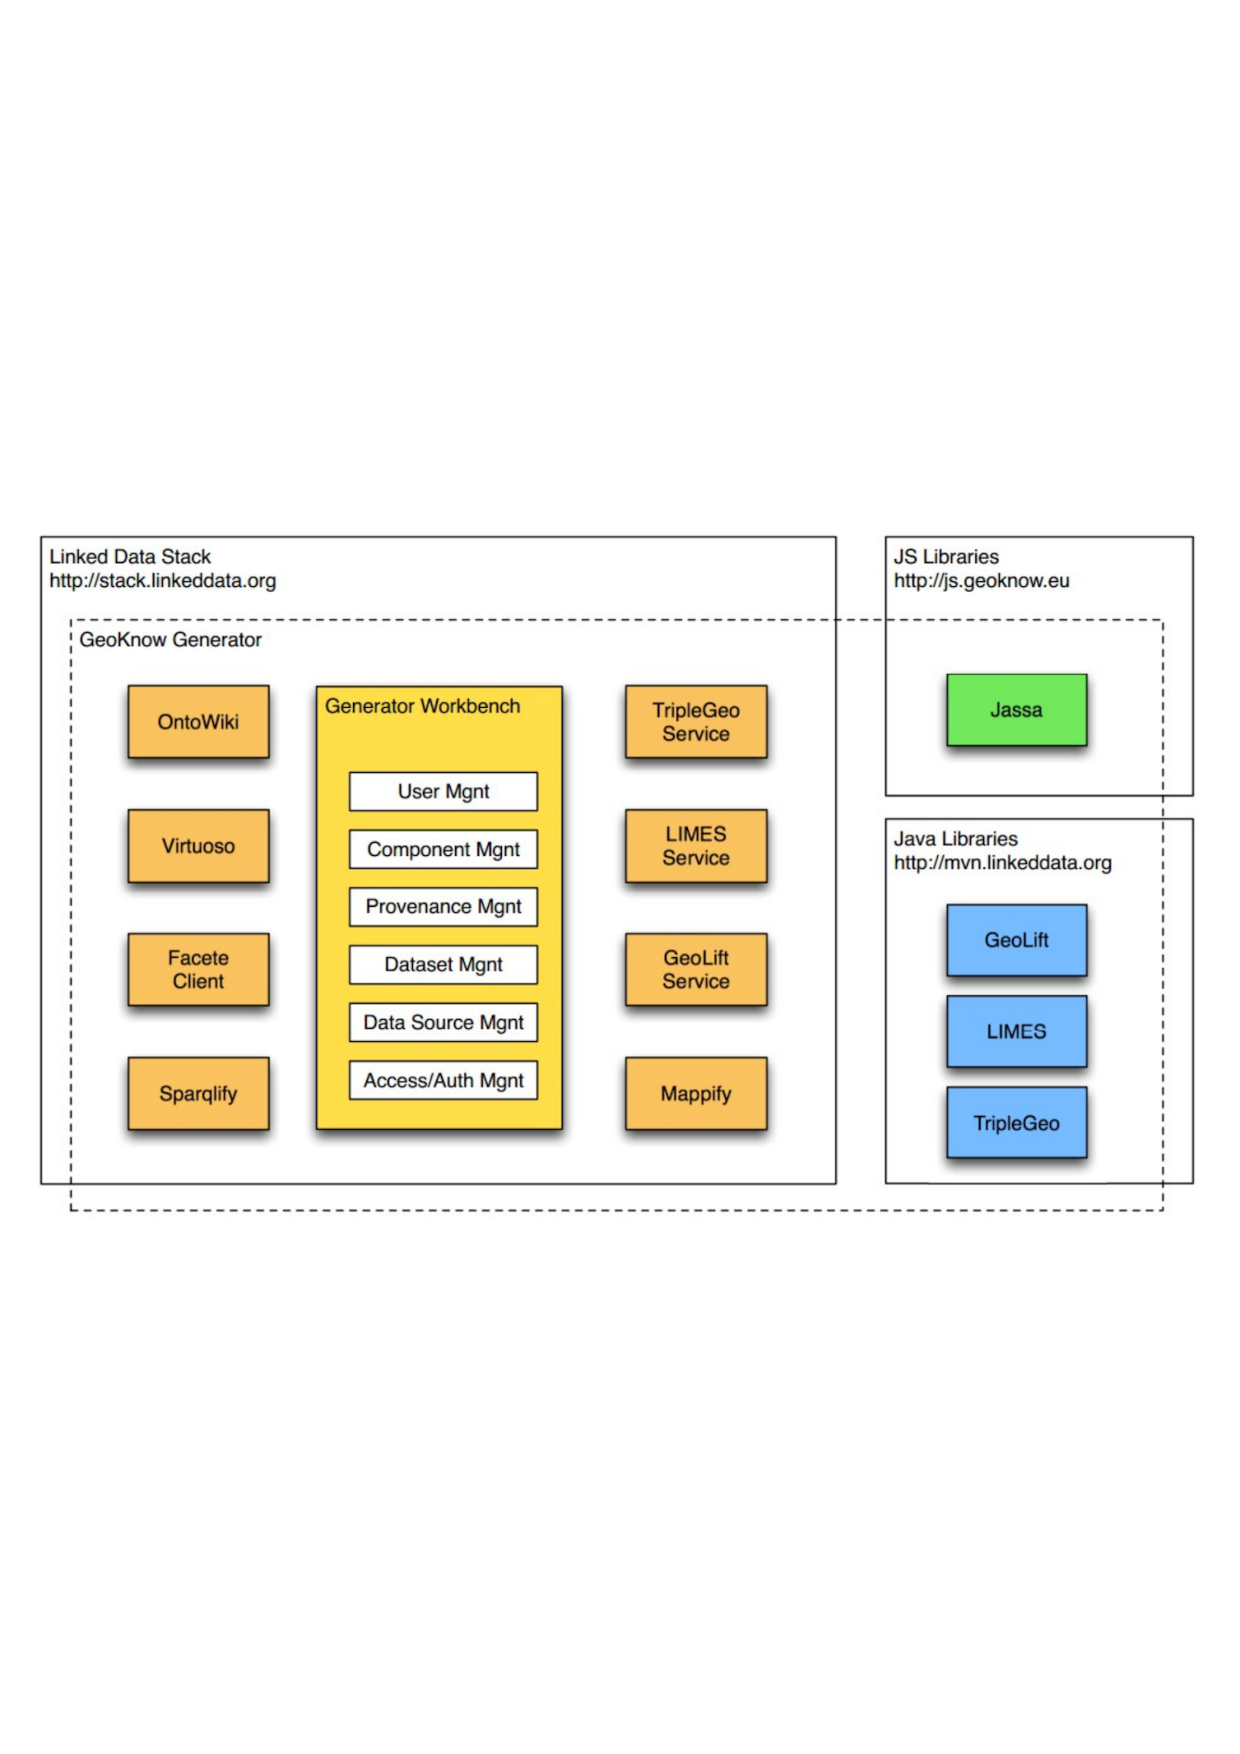
\includegraphics[scale=0.7]{img/geoknow-architecture.pdf}
\label{fig:geoknow}
\vspace{-7cm}
\caption{Architecture of the Geoknow Stack.}

}
\end{figure*}

Below a brief description of the main modules:
\begin{itemize}
\item \textbf{Extraction and Loading:} The module is in charge of loading/importing RDF datasets, extract and convert legacy datasets using extractors/mappers such as TripleGeo (Cf.Section \ref{sec:toolgeo}) and Sparqlify\footnote{\url{http://sparqlify.org/}}. Sparqlify is a SPARQL-SQL rewriter that enables one to define RDF views on relational databases and query them with SPARQL. Currently in alpha state, it powers the Linked-Data Interface of the LinkedGeoData Server and provides access to billions of virtual triples from the OpenStreetMap database.
\item \textbf{Storage and Querying:} The module is powered by Virtuoso 7.0 triple store for querying the datasets.
\item \textbf{Authoring module} integrated the OntoWiki tool \cite{ontowiki14} that facilitates the visual presentation of a knowledge base as an information map, with different views on instance data. It enables intuitive authoring of semantic content, with an inline WYSIWYG editing mode for editing RDF content.

\item \textbf{Linking and Fusion:} To achieve this module, LIMES is the tool integrated in the workbench. LIMES is an abbreviation of the LInk discovery framework for MEtric Spaces, a tool for interlinking resources on the Web of Data\footnote{\url{http://aksw.org/Projects/LIMES.html}}. It implements time-efficient approaches for large-scale link discovery based on the characteristics of metric spaces \cite{ngau11}. It is easily configurable via a web interface or can also be downloaded as standalone tool for carrying out link discovery locally. LIMES can reduce the number of comparisons needed during the mapping process by several orders of magnitude \cite{song13}. The approaches implemented in LIMES include the original LIMES algorithm for edit distances, REEDED for weighted edit distances, HR3, HYPPO, and ORCHID. The algorithms implemented  include the supervised, active and unsupervised versions of EAGLE, COALA and EUCLID \cite{ngon13}.

\item \textbf{Enrichment:} During the enrichment step, the tool \textsc{GeoLift} \cite{geolift14} to enrich geographic content using three techniques: linking, dereferencing and Natural Language Processing (NLP). The code is available at \url{https://github.com/AKSW/GeoLift/}.

\item \textbf{Exploration:} The workflow proposes two tools for this module: \textsc{Mappify} and \textsc{Facet}. The former is a tool for exploring (geographical) Linked Data datasets on the Web, while the latter allows  to explore the specific slice of data named ``facet''  of a Linked Data endpoint in a graphical way, by defining set of constraints on properties of the database. Once the facet is define, the information in the facet can be clicked-through in a tabular interface and visualized on a map. Facete is available at \url{http://144.76.166.111/facete/}.
\end{itemize}

%\todo{add LOD2 work}

\subsection{Comparison between Geoknow Stack and Datalift}
\label{sec:geoknow-datalift}
As described above, Geoknow Stack share similar goals and functionalities with Datalift. However, while the latter is cross-domain and generic, the former is more target for geospatial data. Moreover, Datalift implement connectors for many triple stores, while Geoknow Stack is powered by Virtuoso. Datalift is available in different platforms (Linux, Windows and Mac OS), while the current version of Geoknow can be installed only in Linux. Table \ref{tab:geoknow-datalift} gives more dimensions of both frameworks.

\begin{table}[ht!bp]
    \caption{Comparison of Datalift with GeoKnow Stack} \label{tab:geoknow-datalift}
    \small
    \center
    \begin{tabularx}{\textwidth}{@{}llX@{}}
     %\begin{tabular}{@{}llX@{}}
    \toprule
    \textbf{Features} 		& \textbf{Geoknow Stack } &  \textbf{Datalift} \\
    \toprule
    \texttt{Scope} 	& Geospatial data & Cross-domain/Generic\\
    \midrule
    \texttt{Triple Store} & Virtuoso 7 & Sesame, Virtuoso 6, AllegroGraph\\
    \midrule
    \texttt{Shape2RDF} &  Few models for geometry & More generic approach\\
    \midrule
    \texttt{Interlinking Tool} & LIMES & SILK \\
    \midrule
    \texttt{Publication} & Publish directly in a graph & Export dump data in CSV, Turtle, NTriples\\
    \midrule
    \texttt{Access Control} & N/A & Security Access Module\\
    \midrule
    \texttt{Installation} & Expert level & One-click\\
    \midrule
    \texttt{Platform} & Linux & Multi-platform\\
    \midrule
    \texttt{Deployment Environment} & N/A & IGN, INSEE\\
    \midrule
    \texttt{Provenance} & Partially (user) & Tracking PROV for each project\\
    \midrule
    \texttt{Visualization} & Facete, Mappify  & Sgvizler, RDFViz\\
    \midrule
    \texttt{Access Control} & N/A & Security Access Module\\
    \midrule
    \texttt{Authoring} & Wiki integrated & N/A\\
    \bottomrule

    % \end{tabular}
    \end{tabularx}
    \end{table}


\section{Publishing French Authoritative Datasets} \label{sec:publishing}

In this section, we provide our contribution on the process of publishing different datasets from the French National Mapping agency and OSM-France. We detailed the workflow starting from the conversion of source files, their modeling using the vocabularies implemented, the interconnection with relevant data sources. We conclude this section by showing the current status of the French LOD cloud according to our contributions so far.

\subsection{Publishing French Administrative Units (GeoFla)} \label{sec:geofla}
As a dataset dedicated to administrative units, GEOFLA\circledR is very likely to be reused by other datasets, either by reusing directly its URIs for georeferencing needs, or by reusing its description of administrative units - labels, properties and geometries - for interlinking purposes.

\subsubsection{Data conversion}
\label{sec:dconversion}
Geofla  is delivered as a set of 4 shapefiles  that describe the boundaries and properties of administrative units of mainland France (for CRS reasons, overseas territories are delivered within different shapefiles) : communes, cantons, arrondissements and departements. For the sake of our application, we have generated another shapefile describing regions by aggregating the geometries of the instances of departments based on their region's foreign key value. This  dataset is updated every year.  Publishing this data in RDF with unique identifiers on the Web will ease the interlinking with some existing datasets describing French boundaries in the wild. We follow a two steps conversion: we use the SHP2RDF module of Datalift to obtain a raw RDF from shapefiles, and the RDF2RDF module of Datalift  using a set of SPARQL construct queries\footnote{ \url{https://github.com/gatemezing/ign-iswc2014/tree/master/rdf2rdf}} for getting a refined RDF datasets using suitable vocabularies.

\subsubsection{URI design policy} \label{sec:urigeofla}

One of the requirements to publish data is to have unique ids and stable URIs\footnote{\url{http://www.w3.org/TR/ld-bp/}} . Since our legacy databases have unique IDs to refer to the objects, we had to make sure they were unique at Web level. Thus, the base scheme for vocabularies URIs is: \url{http://data.ign.fr/def/}. Besides, the base schema for identifying a real world resource uses \url{http://{BASE}/id/}. For example, IGN main buildings  are located in the commune with the URI \url{rgeofla:commune/94067}, corresponding to Saint-Mand\'{e}, and \url{rgeofla:departement/94} corresponds to the department ``Val de Marne'' to which the commune belongs.
We had to make choices based on the set of best practices related to URI design\footnote{\url{http://www.w3.org/TR/ld-bp/\#HTTP-URIS}} which should guarantee stable and human readable identifiers.


\subsubsection{Interlinking with existing GeoData} \label{sec:mapping}
We interlinked our datasets with NUTS, DBpedia FR\footnote{\url{http://fr.dbpedia.org/}} and GADM datasets. SILK \cite{jentzsch2010silk} is used to interlink the departments in our dataset with departments in DBpedia FR, using labels and INSEE Code. We obtained $93$ matches (all correct) while three are missing for the departments 07, 09 and 75\footnote{\url{https://github.com/gatemezing/ign-iswc2014/tree/master/interlinking/matched}}. The
LIMES tool\footnote{\url{https://github.com/AKSW/LIMES.}} is then used to perform the rest of the interlinking tasks \cite{ngon13} with the trigrams function based on the labels with restriction to France.

\begin{itemize}
 \item Geofla-RDF with DBpedia FR: \textbf{23 252} links obtained. This results show the missing of nearly 13 435 communes not correctly typed in DBpedia FR as \texttt{Spatial Feature} or \texttt{Place}, or not having a French Wikipedia entry.
 \item Geofla-RDF with GADM (8 314 443 features): \textbf{70} links obtained: 10 communes, 51 departments and 9 regions. The property \texttt{gadm:in\_country} is used to restrict the interlinking to France. E.g.: The city of Saint-Alban in Quebec is a commune in France.
 \item Geofla-RDF with NUTS (316 236 triples): Using a \textit{``naive''} script with \texttt{trigrams} function on \texttt{geofla:Commune/rdfs:label} and \texttt{spatial:Feature/ramon:name} reveal two odd results located in Germany and Switzerland. The latter being the \textit{JURA } and the former named \textit{``Celle''}.  In order to remove those odd effects, we add another restrictions based on \textsf{ramon:code} by filtering the ones located in France (136 features) . The final matchings give a total of \textbf{105} correct links: 14 communes, 75 departments and 16 regions.
\end{itemize}

The above results show good precision of the matching algorithm (score above 0.98) and a rather low recall value with DBPedia-FR (0.627). The few number of matched entities is likely due to the low coverage of French features  in the datasets.


\begin{table}[!htbp]
\centering{

\begin{tabular}{lccl}
\specialrule{1pt}{1pt}{1pt}
 \textbf{Datasets}	 & Precision & Recall & F1-score \\   \specialrule{1pt}{1pt}{1pt}
 NUTS & $0.98$ & $1$ & $0.90$   \\
 GADM & $1$ & $0.86$ & $0.92$  \\
 DBpedia-FR & $1$ & $0.627$ & $0.77$
 \\ \specialrule{1pt}{1pt}{1pt}
\end{tabular}
\caption{Evaluation results in the interlinking process. }
\label{tab:mappins}
}
\end{table}

The SPARQL endpoint for the French Administrative dataset is available for querying at \url{http://data.ign.fr/id/sparql}.

%(\texttt{[filter (contains(ramon:code), ``FR'')]})
%leading to \texttt{nuts:DE931 sameAs geoign:commune/41030}



\subsection{Publishing  French Gazetteer} \label{sec:bdtopo}

In this section, we present some first tests of converting BDTOPO\circledR ~into RDF and interlinking with LinkedGeoData using LIMES. The results confirm the need for geographic publishers to publish georeference data on the Web.
%We  then discuss some challenges related to updating the datasets, versioning and license policies.

\paragraph{Data conversion, URIs and Interlinking:}
Shapefiles are converted into RDF using the same two conversion process as for GEOFLA\circledR. The URIs for each resource follow the pattern: \url{rtopo:CLASS/ID} for the feature, while  \url{rtopo:geom/CLASS/ID} is used to reference the geometry of the resource.
The gazetteer dataset in RDF is part of BD TOPO\circledR ~database consisting of  1,137,543 triples (103,413 features). We chose LinkedGeoData (LGD)
\footnote{\url{http://linkedgeodata.org/sparql}} to perform the alignments using the main class \texttt{lgdo:Amenity}\footnote{\url{http://linkedgeodata.org/ontology/}} (5,543 001 triples), as they are closed to the features contained in the gazetteer. We perform the interlinking on the geometries using the \texttt{hausdorff} metric of LIMES tool. A total of \textbf{654} alignments was obtained above the threshold ($0.9$). This relatively low number of hits can be explained by the coverage of French data in LGD, and the subset of BDTOPO\circledR  ~used for the interlinking. Table~\ref{tab:lgdmapping} provides details of the alignments with subclasses of Amenity.

\begin{table}[!htbp]
\centering{

\begin{tabular}{lr}
\specialrule{1pt}{1pt}{1pt}
 \textbf{LGD Class}	& 	\textbf{\#links matched}	  \\ \specialrule{1pt}{1pt}{1pt}
\textsf{lgdo:Shop} 	   & 252  \\
\textsf{lgdo:TourismThing} &  30 \\
\textsf{lgdo:Craft} &  3 \\
\textsf{lgdo:AerowayThing} &  37 \\
\textsf{lgdo:AerialwayThing} &  11 \\
\textsf{lgdo:EmergencyThing} &  56 \\
\textsf{lgdo:HistoricThing} &  257 \\
\textsf{lgdo:MilitaryThing} &  8
		\\ \specialrule{1pt}{1pt}{1pt}
\end{tabular}
\caption{Interlinking results using the Hausdorff metric of LIMES tool between LinkedGeoData and toponyms in the French Gazetteer}
\label{tab:lgdmapping}
}
\end{table}


\subsection{Publishing Addresses of OSM-France in RDF}
\label{sec:bano2rdf}
OpenStreetMap France is working on providing the location addresses of France in different formats: CSV, ShapeFiles in a collaborative and open source fashion. The BANO project contains already 15 millions of indirect georeferencing locations. The geometries are POINTs and use WGS84 CRS. One of the requirement is to provide a RDF-ize version of the data, enriching the dataset with external/existing relevant ones. The goal of \textsc{Bano2RDF} with three basic requirements:
\begin{description}
\item [\ding{117}~Requirement 1 (Req1)-Model:] Model the existing data according to an existing vocabulary, generic enough to cover the scope of the existing dataset.
\item[\ding{117}~Requirement 2 (Req2)-Provenance:] Add relevance metadata on the published dataset  such as provenance, spatial coverage, licensing, authorship, etc.
\item[\ding{117}~Requirement 3 (Req3)-Stable URIs]: Define a policy to provide and ensure stable URIs for identifying uniquely each address entity on the Web.
\item[\ding{117}~Requirement 4 (Req4)-Interconnection:] Find relevant dataset already published on the Web to which interconnect for better discoverability.

\item[\ding{117}~Requirement 5 (Req5)-Access to data:] Provide primarily a frequent dump of the dataset in RDF.

\item[\ding{117}~Requirement 6 (Req6)-GeoSPARQL interoperability:] Provide different representations of geometries of locations that are interoperable with GeoSPARQL standard.

\end{description}

%\todo{find URI for 450, route des chappes, biot in bano2rdf as sample}
%http://id.osmfr.org/bano/01001A008W-1 {codeinsee + code +numrue}

Based on the above requirements, the Location Core Vocabulary \cite{locnvocab} is used in an \textit{ad-hoc} script\footnote{\url{https://github.com/osm-fr/bano/blob/master/out/csv2ttl.py}} to convert CSV data into RDF. URIs used to identify objects are of the form: \url{http://id.osmfr.org/bano/INSEE-CODE+FANTOIR-CODE+Street-Number}. For example, the location corresponding to EURECOM in SophiaTech (\textit{450, route des chappes, biot, 06410 Biot, FRANCE}) is identified by the URI \\
\texttt{<http://id.osmfr.org/bano/060180238L-450>}. Moreover, the property \\ \texttt{locn:location} links to French Statistic dataset\footnote{\url{http://id.insee.fr}} for communes in France. Metadata are inserted at the beginning of the dataset in RDF corresponding to a department, using vocabularies to model license, spatial coverage of the data (i.e., \texttt{dcat}, \texttt{dcterms}, \texttt{foaf}). The extract below represents the metadata for the department of ``ALPES-MARITIMES'' which the commune of Biot belongs:

\begin{verbatim}
<http://www.openstreetmap.fr/bano/data/> a dcat:Catalog ;
		dcterms:title "Donnees des adresses du projet BANO en RDF"@fr ;
		dcterms:description "Le projet BANO en RDF de Base d'Adresses Nationale
		Ouverte par OpenStreetMap France."@fr ;
		foaf:homepage <http://openstreetmap.fr/bano> ;
		dcterms:language "fr" ;
		dcterms:license <http://www.opendatacommons.org/licenses/odbl/> ;
		dcterms:publisher <http://www.openstreetmap.fr/> ;
		dcterms:issued "2014-05-14"^^xsd:date ; # data issued
		dcterms:modified "2014-08-21"^^xsd:date ; #last modification
		dcterms:spatial <http://id.insee.fr/geo/departement/06>,
		 <http://id.insee.fr/geo/pays/france> .
		
\end{verbatim}

Geometries are provided in three different representations: W3C WGS84, typed literal in WKT and geo URI; all using the property \texttt{loc:geometry}. Currently, the dataset is mostly available as dump files at \url{http://www.openstreetmap.fr/bano/data/}. However, an experimental endpoint has been set up to query at \url{http://eventmedia.eurecom.fr/sparql } with the named graph \url{http://data.osm.fr/bano/}, consisting of nearly 170 million triples.

\paragraph{Interconnection with LinkedGeoData:}
Regarding the interconnection with more existing geodata, first results of mappings with LinkedGeoData amenities using LIMES tool against three big cities of France (Paris, Lyon and Marseille). The dataset is loaded in an endpoint, and the postal code is used to filter the relevant location address. Furthermore, the \textsc{Hausdorff} function is used on the geometry (polygons) of the target and source datasets, with a threshold of 0.97, i.e, we consider \textit{``very closed''} resources with 30 meters distances. Listing \ref{scriptLIMES} shows the configuration used for finding corresponding buildings of LinkedGeoData in Bano2RDF dataset.

\lstset{basicstyle=\scriptsize, backgroundcolor=\color{white}, frame=shadowbox, caption= {LIMES script used to interconnect Bano2RDF dataset located in the region of Marseille with Building in LinkedGeoData.}, label=scriptLIMES, captionpos=b}
\begin{lstlisting}
<LIMES>
	
	<PREFIX>
		<NAMESPACE>http://geovocab.org/geometry#</NAMESPACE>
		<LABEL>geom</LABEL>
	</PREFIX>

	<PREFIX>
     <NAMESPACE>http://www.w3.org/ns/locn#</NAMESPACE>
     <LABEL>locn</LABEL>

    </PREFIX>
	<PREFIX>
		<NAMESPACE>http://www.opengis.net/ont/geosparql#</NAMESPACE>
		<LABEL>geos</LABEL>
	</PREFIX>
	<PREFIX>
		<NAMESPACE>http://linkedgeodata.org/ontology/</NAMESPACE>
		<LABEL>lgdo</LABEL>
	</PREFIX>
	<PREFIX>
      <NAMESPACE>http://www.geonames.org/ontology#</NAMESPACE>
      <LABEL>gn</LABEL>
    </PREFIX>
	<SOURCE>
		<ID>bano2RDF</ID>
		<ENDPOINT>http://eventmedia.eurecom.fr/sparql</ENDPOINT>
		<VAR>?x</VAR>
		<PAGESIZE>5000</PAGESIZE>
		<RESTRICTION>?x a locn:Address</RESTRICTION>
		<RESTRICTION>?x locn:postalCode ?code</RESTRICTION>
		<RESTRICTION>FILTER(regex(str(?code), '690'))</RESTRICTION>
		<PROPERTY>locn:geometry/geos:asWKT RENAME polygon</PROPERTY>
		<TYPE>SPARQL</TYPE>
	</SOURCE>
	<TARGET>
		<ID>linkedgeodata</ID>
		<ENDPOINT>http://linkedgeodata.org/sparql</ENDPOINT>
		<VAR>?y</VAR>
		<PAGESIZE>5000</PAGESIZE>
		<RESTRICTION>?y a lgdo:Building</RESTRICTION>
		<PROPERTY>geom:geometry/geos:asWKT RENAME polygon</PROPERTY>
		<TYPE>SPARQL</TYPE>
	</TARGET>
	
	<METRIC>hausdorff(x.polygon, y.polygon)</METRIC>
	<ACCEPTANCE>
		<THRESHOLD>0.97</THRESHOLD>
		<FILE>bano690xx-lgdBuilding_verynear.nt</FILE>
		<RELATION>lgdo:near</RELATION>
	</ACCEPTANCE>
	<REVIEW>
		<THRESHOLD>0.95</THRESHOLD>
		<FILE>bano690xx-lgdBuilding_place_near.nt</FILE>
		<RELATION>lgdo:near</RELATION>
	</REVIEW>

	<EXECUTION>Simple</EXECUTION>
	<OUTPUT>TAB</OUTPUT>
</LIMES>
	
\end{lstlisting}

Table \ref{tab:bano-gld} shows the first results of the mappings. For each type of amenities in LinkedGeoData, it shows the number of matched resources, and the percentage of the result with respect to the distinct individuals of the category. For example, the mapping reveals $735$ parkings located in Paris (postal code starting with 750). Since there are $250,516$ resources of type ``Parking'' in LinkedGeoData, the percentage is 0.293\%, i.e.,(735/250680)*100.  The table also reveals the low presence of the addresses for French territory in LinkedGeoData. All the results of the mappings are available at \url{https://github.com/gatemezing/bano2rdf-matching}. Shops and restaurants are the resources with most \texttt{owl:sameAs} links between Bano2RDF and LGD datasets.

\begin{table}[ht!b]

        \begin{tabular}{|c|c|c|c|c|c|c|}
            \cline{1-7}
           \multirow{2}{*}{LGData Amenities}  & \multicolumn{2}{|p{2cm}|}{Bano-750xx (248,052)} & \multicolumn{2}{|p{2cm}|}{Bano-130xx (401,404)} & \multicolumn{2}{|p{2cm}|}{Bano-690xx (89,061)}\\
            \cline{2-7}
             & \#matched & \% & \#matched & \% & \#matched & \% \\
            \hline
            \multicolumn{1}{|p{2cm}|}{Building (22,283)} & 05& 0.022 & 12 & 0.053 & 0 & 0  \\
            \hline
            \multicolumn{1}{|p{2cm}|}{Parking (250,516)} & 735 & 0.293 & 625 & 0.24 & 210 & 0.083  \\
            \hline
            \multicolumn{1}{|p{2cm}|}{Shop (778,680)} & 21,171 & 2.71 & 8,556 & 1.098 & 3,049 & 0.391  \\
            \hline
            \multicolumn{1}{|p{2cm}|}{School (318,287)} & 883 & 0.277 & 411 & 0.129 & 197 & 0.061  \\
            \hline
            \multicolumn{1}{|p{2cm}|}{PlaceOfWorship (357,445)} & 272 & 0.076 & 193 & 0.053 & 31 & 0.008  \\
            \hline
            \multicolumn{1}{|p{2cm}|}{Restaurant (260,675)} & 13,567 & 5.204 & 2,654 & 1.018 & 1,882 & 0.721  \\
            \hline
            \multicolumn{1}{|p{2cm}|}{PublicBuilding (26,735)} & 97 & 0.362 & 64 & 0.239 & 21 & 0.078  \\
            \hline
            \multicolumn{1}{|p{2cm}|}{PostOffice (87,731)} & 971 & 1.106 & 555 & 0.632 & 173 & 0.197  \\
            \hline
        \end{tabular}

        \caption{Initial mappings of Bano2RDF with LGD amenities resources respectively in Paris, Marseille and Lyon. The links are obtained using LIMES tool with a threshold of .97 using the \texttt{Hausdorff} distance.}
        \label{tab:bano-gld}
    \end{table}


\subsection{Status of French LOD cloud (FrLOD) }
\label{sec:frenchCloud}
%\todo{Summarize here our contributions to the French LOD Cloud. Give some statistics and explain the figure}\\

We summarize in this section our contributions for a \textit{French LOD (FrLOD)} cloud, consisting of the different datasets published in RDF based on best practices for publishing data in 4-5 stars on the Web. Datasets published belong to different domains: geographical, governmental, statistical and educational. A \texttt{void} description of the FrLOD gives details of the different datasets published\footnote{An interactive version can be accessed at \url{http://www.eurecom.fr/~atemezin/work/frenchLOD.svg}}, links and applications/visualizations built on top of them. Figure  \ref{fig:frenchLOD} depicts a static diagram of the FrLOD, while in Table \ref{tab:frLOD} gives an overview of the datasets, number of triples and domains. Altogether, the FrLOD represents 340 million RDF triples, which is nearly \textbf{10\%} of the DBpedia 2014 release\footnote{\url{http://wiki.dbpedia.org/Datasets}}.

\begin{figure}[h!tb]
  \centering{

      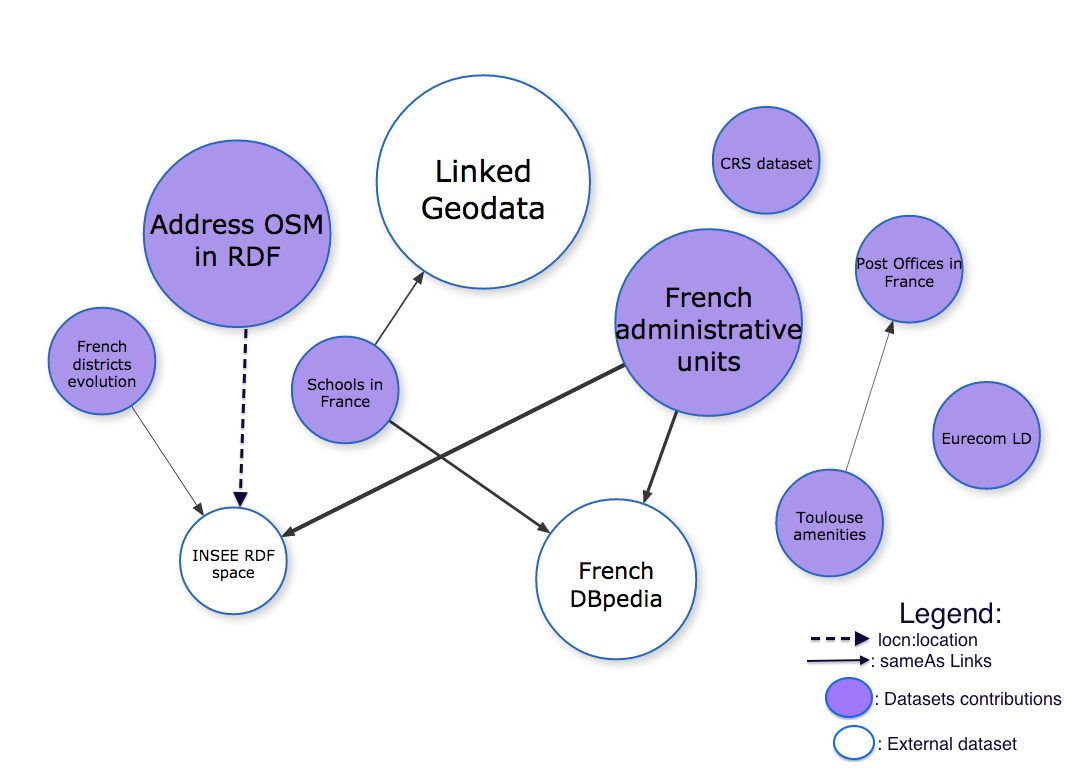
\includegraphics[width=\linewidth]{img/frenchCloud.png}

    \caption{French LOD cloud diagram based on the different datasets published in 4-5 stars. }
    \label{fig:frenchLOD}
  }
\end{figure}

\begin{table}[!htbp]
\centering{

\begin{tabular}{lll}
\specialrule{1pt}{1pt}{1pt}
 \textbf{Dataset}	& 	  \textbf{NbTriples} & \textbf{Domain}\\ \specialrule{1pt}{1pt}{1pt}
French Admin Unit 	   & 173,639,128  & Geography \\
Schools in France 	   & 1,454,564  & Statistics \\
Eurecom LD 	   & 34,651  & Education \\
CRS dataset    & 23, 377  & Government \\
Toulouse Amenities & 963, 618 & Government\\
Bano Project & 163, 723, 230  & Geography \\
French Post Offices & 371, 381 & Government \\
French District Evolution & 150, 356 & Geography \\


		\\ \specialrule{1pt}{1pt}{1pt}
\end{tabular}
\caption{Overview of the content of our contribution to the French LOD Cloud }
\label{tab:frLOD}
}
\end{table}


\section{Evaluation}
\label{sec:geoqueries}

We illustrate in this section different queries making use of geospatial data and geometries functions implemented in three endpoints (virtuoso, owlim, sesame). Within the queries, we use the following points in WGS84, in the the form (longitude latitude): Eurecom, located at (7.0463, 43.6266) and Eiffel Tower, located at (2.2942 48.8628). We perform the time for retrieving the results as well as the expressivity of the types of SPARQL quieries available to users to get the results.

\subsection{Querying LinkedGeodata}
\label{sec:linkedgeodata}

The query below finds public buildings 10 km around Eurecom with their corresponding distance from LinkedGeodata endpoint. In this query, we use the functions of \texttt{st\_distance}, \texttt{st\_intersects} and \texttt{st\_point}. Time used to answer this query is \textbf{341 ms}, monitored by using the time command on \texttt{CURL -g <query>}. The result is listed in Table \ref{tab:lgd-query}

\lstset{basicstyle=\scriptsize, backgroundcolor=\color{white}, frame=shadowbox, caption= {Query on LinkedGeodata endpoint to find all public buildings 10 km around Eurecom building in SophiaTech.}, label=snapshot, captionpos=b}
\begin{lstlisting}
Prefix lgd:<http://linkedgeodata.org/>
Prefix lgdo:<http://linkedgeodata.org/ontology/>

SELECT ?s ?name  (bif:st_distance(bif:st_point(?long, ?lat), bif:st_point(7.0463, 43.6266)) as ?distance)
WHERE
 {
      ?s a lgdo:PublicBuilding ; rdfs:label ?name .
      ?s geo:lat ?lat ; geo:long ?long .
    filter (bif:st_intersects(bif:st_point(?long, ?lat), bif:st_point(7.0463, 43.6266), 10 ))
 }ORDER BY ASC (?distance)
\end{lstlisting}

\begin{table}[!htbp]
\centering{

\begin{tabular}{cl}
\specialrule{1pt}{1pt}{1pt}
 \textbf{s}	& 	  \textbf{distance} \\ \specialrule{1pt}{1pt}{1pt}
\url{http://linkedgeodata.org/triplify/node1645286605} 	   & 1.43949  \\
\url{http://linkedgeodata.org/triplify/node1274078114} &	 4.12131 \\
\url{http://linkedgeodata.org/triplify/node1082377863	} &  5.06445 \\
\url{http://linkedgeodata.org/triplify/node1082377868	} & 	5.14575 \\
\url{http://linkedgeodata.org/triplify/node960122458}	 &  5.54149 \\
\url{http://linkedgeodata.org/triplify/node471974902}	 & 	7.07093 \\
\url{http://linkedgeodata.org/triplify/node2209129663} & 7.59737

		\\ \specialrule{1pt}{1pt}{1pt}
\end{tabular}
\caption{Results of the public buildings 10 km around EURECOM from LinkedGeoData endpoint.}
\label{tab:lgd-query}
}
\end{table}



\subsection{Querying FactForge (OWLIM)}
\label{sec:factforge}

The query below find in FactForge\footnote{\url{http://factforge.net/sparql}} the french departments within the Bounding Box of Eurecom and Eiffel Tower. We use the function \texttt{omgeo:within}. The results\footnote{\url{http://goo.gl/dLc45p}} consist of 36 departments and the query takes \textbf{1.369 s} to be completed.
\begin{verbatim}
PREFIX omgeo: <http://www.ontotext.com/owlim/geo#>
PREFIX geo-ont: <http://www.geonames.org/ontology#>
SELECT DISTINCT ?link ?m
WHERE {
 ?link geo-ont:name ?m.
  ?link geo-ont:featureCode geo-ont:A.ADM2 .
  ?link geo-ont:parentCountry dbpedia:France .
  ?link geo-pos:lat ?lat2 .
  ?link geo-pos:long ?long2 .
 ?link omgeo:within( 43.6266 2.2942 48.8628 7.0463 ) }.

\end{verbatim}

%\todo{make a table to compare the results and comment them}

\subsection{Case of Structured Geometries}
\label{sec:ignsparql}
%Here adapt the use case of French Geofla, and compare with the previous.
 We query data.ign.fr endpoint that contains structured geometries of French departments, powered by Datalift, using the default triple store Sesame. The query finds all the departments containing in the Bounding Box formed by EURECOM and Eiffel Tower. The results consisting of 94 departments is obtained after \textbf{23.496s} when launched against \url{data.ign.fr/id/sparql}. Not all the SPARQL1.1 property paths \footnote{\url{http://www.w3.org/TR/sparql11-query/\#propertypaths}} are fully implemented in Virtuoso endpoints.


 \begin{verbatim}
 SELECT DISTINCT ?name  WHERE {
?dep a geofla:Departement .
?dep rdfs:label ?name .
?dep geom:geometry/geom:centroid ?ct .
?ct geom:coordX ?long ; geom:coordY ?lat.
?dep geom:geometry/geom:polygonMember/geom:exterior/geom:points ?pl .
?pl rdf:type geom:PointsList .
?pl (rdf:rest*/rdf:first)|geom:firstAndLast ?pm .
?pm rdf:type geom:Point .
?pm geom:coordX ?x .
?pm geom:coordY ?y .
FILTER ((?x > 2.2942 && ?x < 7.0463) &&(?y > 43.6266 && ?y < 48.8628)) .
}
 \end{verbatim}


The result in section \ref{sec:ignsparql} suggests that it's possible to reduce the time of querying geographic data by just using standard SPARQL queries without geosptial built-in functions.

\section{Summary}
\label{sec:ch2-summary}
In this chapter, we have surveyed tools for extracting and converting geospatial data in RDF. Then, we described GeomRDF, a tool developed within the Datalift project which goes beyond the state-of-art by providing structured geometries and conform to GeoSPARQL. Moreover, we have described the limitation of existing data models by discussing some recommendations to publishers of geodata on storage aspects. Similarly, an extensive description of Datalift tool used to publish data on the Web has been provided, with special focus of our contribution to build the French LOD cloud with datasets in 4-5 stars according to Linked Data principles. Finally, we have shown some real world use-cases of SPARQL queries making use of either structured geometries or built-in geospatial functions. According to the requirements of the users and the underlying datasets, the user can choose between the simplicity of SPARQL query, with limitations to the endpoint (for e.g., when using built-in geospatial functions of a given endpoint), or the expressivity of the \texttt{geom} vocabulary regardless the endpoint, with a more longest SPARQL query.


The next chapter is about consuming datasets published on the Web, where we explore tools for visualizing data published as LOD, and later propose our approach which is a category-based visualization wizard.
